
In this chapter, the mathematical background of this thesis is presented. Specifically, is introduced the basic notations and definitions of graph theory, as well some mathematical concepts of matrix theory, Lyapunov stability theory and basic theorems of mathematical analysis. In addition, is introduced and the augmented Lagrangian algorithm.

\section{Graph Theory}

\subsection{Basic Definitions}
    \begin{definition}\label{def:2.1}
        \cite{GR2001} A finite graph $\mathcal{G}$ is a non-empty finite set $\mathcal{G} = (\mathcal{V},\mathcal{E},\mathcal{A})$ which is consisted of a finite non-empty set $\mathcal{V}(\mathcal{G})$, a finite non-empty set $\mathcal{E}(\mathcal{G})$ and $\mathcal{A}$ is the incidence matrix of the graph. The set $\mathcal{V}(\mathcal{G})$ contains the vertices (nodes) of the graph, with $|\mathcal{V}| = N$ and the set $\mathcal{E}(\mathcal{G})$ contains the edges of the graph with $|\mathcal{E}| = E$, which connect the vertices. 
    
        If there exists an edge between the vertices $v_i$ and $v_j$, then the vertices are defined as adjacent with the symbol $v_i \sim v_j$.
        \begin{figure}[H]
            \centering
            \begin{minipage}{.5\textwidth}
                \centering
                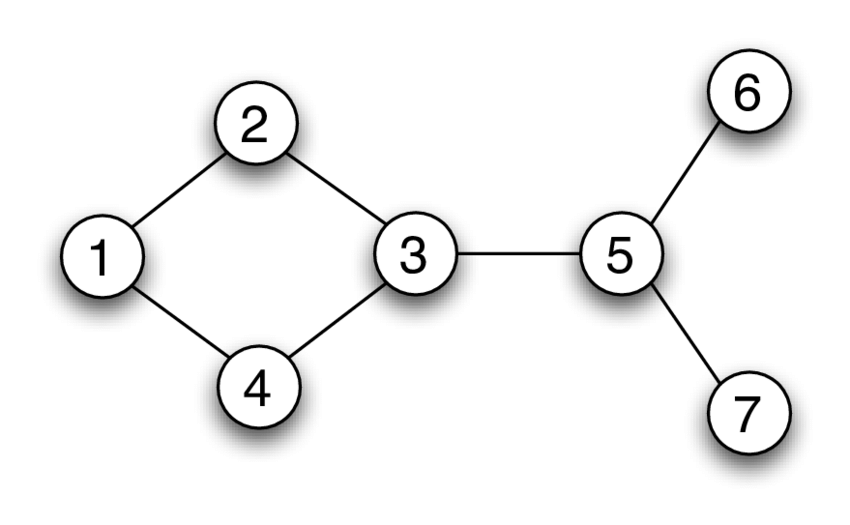
\includegraphics[width=0.8\linewidth]{images/Chapter2/undigraph.png}
                \caption{Undirected graph topology.}
                \label{fig:2.1}
            \end{minipage}%
            \begin{minipage}{.5\textwidth}
                \centering
                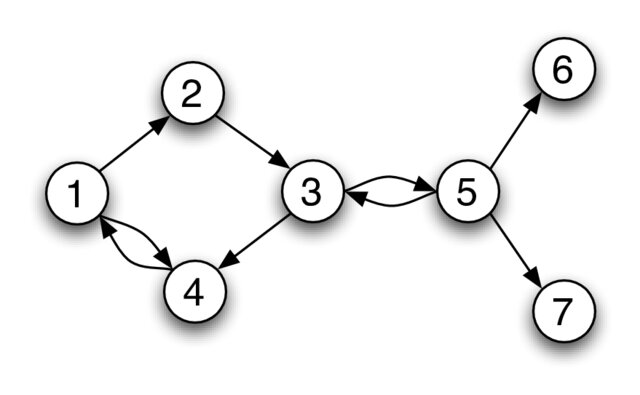
\includegraphics[width=0.8\linewidth]{images/Chapter2/digraph.png}
                \caption{Directed graph topology.}
                \label{fig:2.2}
            \end{minipage}
        \end{figure}
    \end{definition}
    \newpage
     \begin{definition}\label{def:2.2}
         \cite{GR2001} A neighborhood of an $i-$agent is defined as\\ $\mathcal{N}(i) := \left\{ j \in \mathcal{V} \hspace{0.5mm} | \hspace{0.5mm}  (i,j) \in \mathcal{E}\right\} \subset \mathcal{V}$.
     \end{definition}
    
    \begin{definition}\label{def:2.3}
        \cite{GR2001} A path of length $l$ from $\{v_{i_0}, v_{i_1}, ..., v_{i_l}\}$ in a graph is a sequence of $l + 1 $ distinct nodes starting with $v_{i_0}$ and ending with $v_{i_l}$ such that consecutive nodes are adjacent.
    \end{definition}
    
     \begin{definition}\label{def:2.4}
         \cite{GR2001} A cycle is a connected graph where every node has exactly two neighbors.
     \end{definition}
    \begin{definition}\label{def:2.5}
        \cite{GR2001} A graph $\mathcal{G}$ is connected, if for every pair of nodes of $\mathcal{V}(G)$, exists a path which have this pair as an end.
    \end{definition}
    
     \begin{definition}\label{def:2.6}
         \cite{GR2001} If in a graph, in addition to its nodes and edges, exists a function $\mathcal{W}:E \to \mathbf{R}$ where assigns a value in every edge, then the graph $\mathcal{G} = (\mathcal{V}, \mathcal{E}, \mathcal{W})$ is called weighted graph.
        \begin{figure}[H]
            \centering
            \begin{minipage}{.5\textwidth}
                \centering
                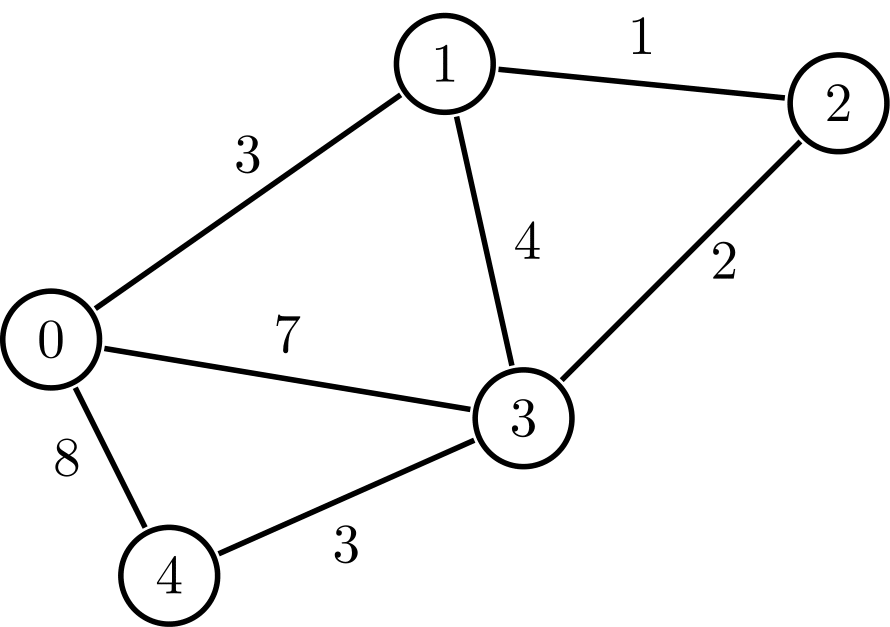
\includegraphics[width=0.8\linewidth]{images/Chapter2/weight graph.png}
                \caption{Undirected weighted \\graph topology.}
                \label{fig:2.3}
            \end{minipage}%
            \begin{minipage}{.5\textwidth}
                \centering
                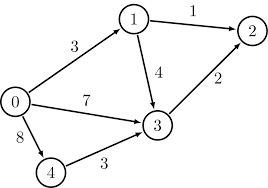
\includegraphics[width=0.8\linewidth]{images/Chapter2/weight digraph.png}
                \caption{Directed weighted \\graph topology.}
                \label{fig:2.4}
            \end{minipage}
        \end{figure}
     \end{definition}
    
\subsection{Graph Matrices}

    In addition to the basic graph notations, matrices can describe them in an algebraic form. Due to the selected algorithm, an incidence matrix is used.
    
    \begin{definition}\label{def:2.7}
        \cite{GR2001} The degree $d(v_i)$ of a node in an undirected graph $\mathcal{G}$ is the total number of nodes which are adjacent to $v_i$.
    \end{definition}
    
    \begin{definition}\label{def:2.8}
        \cite{GR2001} The degree matrix $D$ of an undirected graph $\mathcal{G}$ is a diagonal matrix whose elements are the degree nodes $d(v_i)$. 
    \end{definition}
    
    
    \begin{definition} \label{def:2.9}
        \cite{hong2016decomposing} The incidence matrix $\mathcal{A}$ is a $N \times E$ matrix, which describes the relationship between a node and an edge. In its $i-$th row and $j-$th column has the number of times the $j-$th edge is incident with the $i-$th vertex. Now the matrix is defined as
        
        \begin{equation}\label{eq:2.1.1}
            [\mathcal{A}]_{ev} = \left\{ \begin{matrix}
                1,\hspace{5.0mm} if \hspace{2.0mm}(i,j) \in \mathcal{E}, with \hspace{2.0mm} i > j \hspace{2.0mm} and \hspace{2.0mm} v = i \\
                -1,\hspace{5.0mm} if \hspace{2.0mm}(i,j) \in \mathcal{E}, with \hspace{2.0mm} i > j \hspace{2.0mm} and \hspace{2.0mm} v = j \\
                0,\hspace{20.0mm} otherwise \end{matrix} \right
        \end{equation}
        
    \end{definition}
    
    
    \begin{definition}\label{def:2.10}
        \cite{GR2001} The Laplacian matrix of an undirected graph $\mathcal{G}$ is defined by
        \begin{equation}\label{eq:2.1.2}
            L= D - \mathcal{A}
        \end{equation}
        where $D$ is the degree matrix and $\mathcal{A}$ is the incidence matrix.
    \end{definition}
    
    \begin{definition}\label{def:2.11}
        \cite{hong2016decomposing} The signed Laplacian matrix of a graph $\mathcal{G}$ is defined as
        \begin{equation}\label{eq:2.1.3}
            L_- = \mathcal{A}^T\mathcal{A}
        \end{equation}
    \end{definition}
    
    \begin{definition}\label{def:2.12}
        \cite{hong2016decomposing} The signless Laplacian matrix of a graph $\mathcal{G}$ is defined as
        \begin{equation}\label{eq:2.1.4}
            L_+ = 2D - \mathcal{A}^T\mathcal{A}
        \end{equation}
    \end{definition}
    

\section{Matrix Theory}

    In this section are going to be introduced the basic notations of matrix theory that will be used.
    
    \begin{definition}\label{def:2.13}
        \cite{strang2006linear} Consider a vector field of $\mathbf{R}^n$ and a squared matrix $A \in \mathbf{R}^{n \times n}$. Then, for a vector $x \in \mathbf{R}^n$ and a constant $\lambda \in \mathcal{C}$ holds that
    
        \begin{equation}\label{eq:2.2.1}
            Ax = \lambda x
        \end{equation}
        where $x$ is called eigenvector of matrix $A$ which is related to the eigenvalue $\lambda$.
    \end{definition}
    The matrix $A$ can be inverted, if he does not have a zero eigenvector. The eigenvalues of a matrix are computed from
    
    \begin{equation}\label{eq:2.2.2}
        \chi_A(\lambda) = det(\lambda I_n - A) = 0
    \end{equation}
    This equation is called the characteristic polynomial of the matrix $A$, with the eigenvalues being its roots. The algebraic multiplicity of an eigenvalue $\lambda$ is the multiplicity as a root of the equation (\ref{eq:2.2.2}). The geometric multiplicity of an eigenvalue $\lambda$, is the maximum number of linear independent eigenvectors, which are associated with this eigenvalue.
    
    \begin{theorem}\label{thr:2.1}
        \cite{strang2006linear}  Let $S$ be a matrix of eigenvectors of a given square matrix $A$ and $\Lambda$ be a diagonal matrix with the corresponding eigenvalues on the diagonal. Then, as long as $S$ is a square matrix, matrix $A$ can be written as an eigen decomposition
        \begin{equation}\label{eq:2.2.3}
            A = S\Lambda S^{-1}
        \end{equation}
        where $\Lambda$ is a diagonal matrix. Furthermore, if $A$ is symmetric, then the columns of $S$ are orthogonal vectors. 
    \end{theorem}
    
    \begin{definition}\label{def:2.14}
        \cite{strang2006linear} A matrix $A$ is called semipositive if the quadratic form
        \begin{equation*}
            x^TAx \geq 0, \forall x
        \end{equation*}
        and positive if the quadratic form is
        \begin{equation*}
            x^TAx > 0, \forall \hspace{2.0mm} x  \neq 0
        \end{equation*}
    \end{definition}
    
    \begin{corollary}\label{cor:2.1}
        \cite{strang2006linear} A matrix $A$ is semipositive iff all his eigenvalues are nonnegative. A matrix $A$ is positive if all his eigenvalues are positive.
    \end{corollary}
    
    \begin{definition}\label{def:2.15}
        \cite{strang2006linear} A matrix $ A \in \mathbf{R}^{n\times n}$ is defined as nonnegative if his elements are nonnegative, i.e. $\alpha_{ij} \geq 0$, for $i,j = 1,...,n$.
    \end{definition}
    
    \begin{definition}\label{def:2.16}
        \cite{strang2006linear} The Kronecker product of two matrices $A \in \mathbf{R}^{n\times m}$ and $B \in \mathbf{R}^{p \times q}$, with $\alpha_{ij} = [A]_{ij}$ and $b_{ij} = [B]_{ij}$, is written as $A \otimes B$ and defined as an $np \times mq$ matrix below
    
        \begin{equation} \label{eq:2.2.4}
            A \otimes B = \left[\begin{matrix}
                 \alpha_{11}B & \cdots & \alpha_{1m}B \\
                    \alpha_{21}B & \cdots & \alpha_{2m}B \\
                    \vdots & \vdots & \vdots \\
                    \alpha_{n1}B & \cdots & \alpha_{nm}B
            \end{matrix} \right]
        \end{equation}
    \end{definition}
    The properties of the Kronecker product are presented below
    
    \begin{equation*}
            A \otimes (B + C) = A \otimes B + A \otimes C
    \end{equation*}
    \begin{equation*}
        (kA) \otimes B = A \otimes (kB) = k(A \otimes B)
    \end{equation*}
    \begin{equation*}
        (A \otimes B) \otimes C = A \otimes (B \otimes C)
    \end{equation*}
    \begin{equation*}
         A \otimes 0 = 0 \otimes A = 0
    \end{equation*}
    where matrices $A,B,C$ have the appropriate dimensions, $0$ is the zero matrix and $k$ is constant.
    

\section{Mathematical Analysis}
    
    In this section are presented the basic notations, theorems and definitions of mathematical analysis. Specifically of real analysis, functional analysis and convex and non-Convex analysis.
    \begin{definition}\label{def:2.17}
        \cite{folland2013real} A continuous function $a:\mathbf{R}_+ \to [0,\infty)$ is a class $\mathcal{K}$ \\function if
        \begin{itemize}
            \item $a \in C^0(\mathbf{R}_+)$
            \item it is strictly increasing in $\mathbf{R}_+$
            \item $a(0) = 0$
        \end{itemize}
    \end{definition}
    \begin{definition}\label{def:2.18}
        \cite{folland2013real} A continuous function $a:\mathbf{R}_+ \to [0,\infty)$ is a class $\mathcal{K}_{\infty}$ \\function if
        \begin{itemize}
            \item $a \in C^0(\mathbf{R}_+)$
            \item it is strictly increasing in $\mathbf{R}_+$
            \item $a(0) = 0$
            \item $\lim_{s \to \infty} a(s) = \infty$
        \end{itemize}
    \end{definition}
    \begin{definition}\label{def:2.19}
        \cite{folland2013real} A continuous function $a: \mathbf{R_+} \times \mathbf{R_+} \to \mathbf{R_+}$ is a class $\mathcal{KL}$ function if
        \begin{itemize}
            \item $a(\cdot, t)$ is strictly increasing in $\mathbf{R_+}$, $\forall t \geq 0$
            \item $a(s,\cdot)$ is strictly decreasing in $\mathbf{R_+}$, $\forall s \leq 0$
            \item $\lim_{t \to \infty} a(s,t) = 0, \forall s \geq 0$
            \item $a(0,t) = 0, \forall t \geq 0$
        \end{itemize}
    \end{definition}
    
    \begin{definition}\label{def:2.20}
        \cite{HK2001} A continuous function $W: \mathbf{R}^n \to \mathbf{R}$ is positive defined iff
        \begin{itemize}
            \item $W(0) = 0$
            \item $W(x) > 0$, \hspace{2.0mm} $\forall x \in \mathbf{R}^n - \{0\}$
            \item exists $r > 0$, such that $\inf_{||x|| \geq r} W(x) > 0$
        \end{itemize}
    \end{definition}
    
    \begin{definition}\label{def:2.21}
        \cite{HK2001} Young inequality is defined as
        \begin{equation}\label{eq:2.3.1}
            a \cdot b \leq \frac{\epsilon}{2}a^2 + \frac{1}{2\epsilon}b^2, \forall a,b \in \mathbf{R}, \forall \epsilon > 0
        \end{equation}
    \end{definition}
    
    \begin{definition}\label{def:2.22}
        \cite{folland2013real} Assume that $p$ and $q$ are in the open interval $(1,\infty)$ with $1/p + 1/q = 1$. Hölder's inequality is defined as
        \begin{equation}\label{eq:2.3.2}
            \left(\sum_{i = 1}^{n} |a_i b_i|\right) \leq \left(\sum_{i = 1}^{n} |a_i|^p\right)^{1/p} \left(\sum_{i = 1}^{n} |b_i|^q\right)^{1/q} 
        \end{equation}
        if $|a_i| = 1$ then
        \begin{equation*}
            \left(\sum_{i = 1}^{n} |a_i b_i|\right) \leq \left(\sum_{i = 1}^{n} |a_i|^p\right)^{1/p} \left(\sum_{i = 1}^{n} |b_i|^q\right)^{1/q}\leq n^{1-p}\left(\sum_{i = 1}^{n} |b_i|^p\right)
        \end{equation*}
    \end{definition}
    
    \begin{definition}\label{def:2.23}
        \cite{JBI1991} A function $f \in C^1({\mathbf{R}^n})$ is called $L-$smooth if satisfies the below inequality, \hspace{1.0mm}$\forall x_1,x_2 \in \mathbf{R}^n$:
        \begin{equation}\label{eq:2.3.3}
            ||\nabla f(x_1) -\nabla f(x_2)|| \leq L ||x_1 - x_2||
        \end{equation}
        or
        \begin{equation}\label{eq:2.3.4}
            |f(x_1) - f(x_2) - \nabla f(x_2)^T(x_1 - x_2)| \leq \frac{L}{2}||x_1 - x_2||^2
        \end{equation}
    \end{definition}
    
    \begin{definition}\label{def:2.24}
        \cite{JBI1991} A function $f \in C^1({\mathbf{R}^n})$ is called convex, if \hspace{1.0mm}$\forall x_1,x_2 \in \mathbf{R}^n$:
        \begin{equation}\label{eq:2.3.5}
            f(x_1) - f(x_2) \geq f(x_2)^T(x_1 - x_2) 
        \end{equation}
    \end{definition}
    
    \begin{definition}\label{def:2.25}
        \cite{JBI1991} A function $f \in C^1({\mathbf{R}^n})$ is called $\sigma-$strongly convex, with $\sigma > 0$, if \hspace{1.0mm}$\forall x_1,x_2 \in \mathbf{R}^n$:
        \begin{equation}\label{eq:2.3.6}
            f(x_1) - f(x_2) - f(x_2)^T(x_1 - x_2) \geq \frac{\sigma}{2}||x_1 - x_2||^2
        \end{equation}
        if $f \in C^2({\mathbf{R}^n})$, is strongly convex and smooth then
        \begin{equation}\label{eq:2.3.7}
            \sigma I_n \preceq \nabla^2 f(x) \preceq LI_n
        \end{equation}
        where $I_n \in \mathbf{R}^{n \times n}$ is the unit matrix with size $n$. If $f(x_1) - f(x_2) - f(x_2)^T(x_1 - x_2) \geq 0$, then from (\ref{eq:2.3.4}) and (\ref{eq:2.3.6}) is obtained:
        \begin{equation}\label{eq:2.3.8}
            \frac{\sigma}{2}||x_1 - x_2||^2 \leq f(x_1) - f(x_2) - f(x_2)^T(x_1 - x_2) \leq \frac{L}{2}||x_1 - x_2||^2
        \end{equation}
    \end{definition}
    
    \begin{definition}\label{def:2.26}
        \cite{JBI1991} A function $f \in C^1({\mathbf{R}^n})$ is called Lipschitz, if  \hspace{1.0mm}$\forall x_1,x_2 \in \mathbf{R}^n$ and a constant $\mathbf{L} \geq 0$:
        \begin{equation}\label{eq:2.3.9}
            ||f(x_1) - f(x_2)|| \leq \mathbf{L} ||x_1 - x_2||
        \end{equation}
    \end{definition}
        
    \begin{definition}\label{def:2.27}
        \cite{JBI1991} A function $f(x)$ is called locally Lipschitz in $\mathcal{D} \subset \mathbf{R}^n$, if every point of $\mathbf{D}$ has an area $\mathbf{D}_0$ which satisfies the Lipschitz condition for a Lipschitz constant $\mathbf{L}_0$. 
    \end{definition}
    
    \begin{definition}\label{def:2.28} 
        \cite{JBI1991} A function $f(x)$ is called globally Lipschitz if it is Lipschitz on $\mathbf{R}^n$.
    \end{definition}
    
    \begin{theorem}\label{thr:2.2}
        \cite{ZSCSP} If $f:R^n \to  R$ is a Lipschitz continuously differentiable on a convex set $\mathcal{C}$\hspace{1.0mm} ($f \in C^1(\mathcal{C})$) with some Lipschitz constant $\mathbf{L}$, then $\phi(x) = f(x) - \frac{1}{2}ax^Tx$ is a convex function on $\mathcal{C}$ for every $a \leq -\mathbf{L}$.
    \end{theorem}

\section{Lyapunov Stability Theory}

    Lyapunov theory was invented from the Russian mathematician Aleksandr Lyapunov, in order to study the stability of dynamical systems. Through his findings, he was able to conclude if a dynamical system is either stable or unstable. The basic concept of stability theory is the definition of a suitable scalar function, which is analyzed to evaluate its properties.

    Consider the $n-$dimensional system

    \begin{equation}\label{eq:2.4.1}
        \dot{\boldsymbol{x}} = f(\boldsymbol{x})
    \end{equation}
    where $f: \mathcal{D} \to \mathbf{R}^n$ is locally Lipschitz over a domain $\mathcal{D} \subset \mathbf{R}^n$. Suppose $\boldsymbol{x}^*$ is an equilibrium point of (\ref{eq:2.4.1}); that is $f(\boldsymbol{x}^*) = 0$.

    \begin{definition}\label{def:2.29}
        \cite{HK2001} Let $f(x)$ be a locally Lipschitz defined over a domain $\mathcal{D} \subset \mathbf{R}^n$, which contains the origin, and $f(0) = 0$. The equilibrium point $x^* = 0$ 0f (\ref{eq:2.4.1}) is
        \begin{itemize}
            \item stable if for each $\varepsilon > 0$ there is $\delta > 0$ (dependent on $\varepsilon$) such that
                \begin{equation*}
                    ||x(0)|| < \delta \Rightarrow  ||x(t)|| < \varepsilon, \forall t \geq 0
                \end{equation*}
            \item unstable if it is not stable.
            \item asymptotically stable if it is stable and $\delta$ can be chosen such that
                \begin{equation*}
                    ||x(0)|| < \delta \Rightarrow \lim_{t \to \infty} x(t) = 0
                \end{equation*}
            \item exponentially stable if there exists $\delta, M, \sigma$ such that
            \begin{equation*}
                ||x(0)|| < \delta \Rightarrow ||x(t)|| \leq Me^{-\sigma t}||x(0)||, \hspace{1.0mm} \forall t \geq 0
            \end{equation*}
        \end{itemize}
    \end{definition}
    

    \begin{definition}\label{def:2.30}
        \cite{HK2001} Consider a function $V: \mathbf{R}^n \to R$, which:
        \begin{itemize}
            \item $V(0) = 0$
            \item $V(x) > 0$, $\forall x \neq 0$
        \end{itemize}
        then it is a positive define function. This function is called Candidate Lyapunov function.
    \end{definition}

    \begin{definition}\label{def:2.31}
        \cite{HK2001} A Lyapunov function $V: \mathbf{R}^n \to R$ is called radially unbounded, if $\forall M > 0$ the set $\{x\in\mathbf{R}^n: \hspace{2.0mm} V(x) \leq M\}$ is bounded, or
        \begin{equation*}
            \lim_{||x|| \to +\infty} V(x) = +\infty
        \end{equation*}
    \end{definition}

    \begin{theorem}\label{thr:2.4}
        \cite{HK2001} Consider a positive defined function $V \in C^1(\mathbf{R}^n)$. Consider an open set $\mathcal{D} \subset \mathbf{R}^n$, with the $0$ inside it such that
        \begin{equation*}
            \nabla V(x) f(x)\leq 0, \forall x \in \mathcal{D}
        \end{equation*}
        then, $0 \in \mathbf{R}^n$ is stable for the system of (\ref{eq:2.4.1}).
    \end{theorem}
    
    
    \begin{theorem}\label{thr:2.5}
        \cite{HK2001} Consider a positive defined function $V \in C^1(\mathbf{R}^n)$. Consider an open set $\mathcal{D} \subset \mathbf{R}^n$, with the $0$ inside it such that
        \begin{equation*}
            \nabla V(x) f(x) < 0, \forall x \in \mathcal{D}, \forall x \neq 0
        \end{equation*}
        then, $0 \in \mathbf{R}^n$ is asymptotically stable for the system of (\ref{eq:2.4.1}).
    \end{theorem}
    
    \begin{definition}\label{def:2.32}
        \cite{HK2001} The equilibrium point of (\ref{eq:2.4.1}) is
        \begin{itemize}
            \item uniformly bounded if there exists a positive constant $c$, independent of $t_0 \geq 0$, and for every $a \in (0,c)$, there exists $\beta = \beta(a) > 0$, independent of $t_0$, such that
            \begin{equation}\label{eq:2.4.2}
                ||x(t_0)|| \leq 0 \Rightarrow ||x(t)|| \leq \beta, \forall t \geq t_0
            \end{equation}
            \item globally uniformly bounded if (\ref{eq:2.4.2}) holds for arbitrarily large $a$.
            \item uniformly ultimately bounded with ultimate bound $b$ if there exists positive constants $b$ and $c$, independent of $t_0 \geq 0$, and for every $a \in (0,c)$, there is $T = T(a,b) \geq 0$, independent of $t_0$, such that
            \begin{equation}\label{eq:2.4.3}
                ||x(t_0)|| \leq a \Rightarrow ||x(t)|| \leq b, \forall t \geq t_0 + T
            \end{equation}
            \item globally uniformly ultimately bounded if (\ref{eq:2.4.3}) holds for arbitrarily large $a$.
        \end{itemize}
    \end{definition}
    

    \begin{lemma}\label{lem:2.1}
        \cite{HK2001} Let $V: \mathcal{D} \to \mathbf{R}$ be a continuous positive function defined inside the domain $\mathcal{D} \subset \mathbf{R}^n$ that contains the origin. Let $B_r \subset \mathcal{D}$ for some $r > 0$. Then, there exist class $\mathcal{K}$ functions $a_1$ and $a_2$, defined on $[0,r]$, such that
        \begin{equation}\label{eq:2.4.4}
            a_1(||x||) \leq V(x) \leq a_2(||x||)
        \end{equation}
        $\forall x \in B_r$. If $\mathcal{D} = \mathbf{R}^n$, the functions $a_1$ and $a_2$ will be defined on $[0, \infty)$ and the foregoing inequality will hold $\forall x \in \mathbf{R}^n$. Moreover, if $V(x)$ is radially unbounded, then $a_1$ and $a_2$ can be chosen to belong to class $\mathcal{K}_{\infty}$.
    \end{lemma}
        

\section{Augmented Lagrangian Algorithm}

Augmented Lagrangian Algorithms have a primal dual multiplier form, \cite{bertsekas2015incremental}, which minimize the summation of the cost function with respect to the constraints of the problem. The algorithm which will be used in this dissertion is Prox-GPDA, \cite{pmlr-v70-hong17a,hong2016decomposing}, which is a proximal form of the classic augmented Lagrangian algorithm with an added proximal term. Consider the following optimization problem

\begin{equation}\label{eq:2.5.1}
    \min_{x \in \mathbf{R}^n} g(x) = \sum_{i = 1}^{N} f_i(x)
\end{equation}
where $f_i(x):\mathbf{R}^n \to \mathbf{R}$, $i\in \{1,...,N\}:= [N]$ are the nonconvex local cost functions of each agent, which are assumed to be smooth and has Lipschitz continuous gradients. Suppose the agents are connected with an undirected graph which is defined in \ref{def:2.1}. Each agent can only exchange information with his neighbor, defined as in \ref{def:2.2} with $|\mathcal{N}_i| = d_i$. The distributed version of problem (\ref{eq:2.5.1}) is

\begin{equation}\label{eq:2.5.2}
    \min_{x_i \in \mathbf{R}^n} f(x) := \sum_{i = 1}^{N} f_i(x_i),\hspace{1.0mm} s.t.\hspace{1.0mm} x_i = x_j,\hspace{1.0mm} \forall (i,j) \in \mathcal{E}
\end{equation}

It is clearly that the problem (\ref{eq:2.5.2}) is equivalent to the problem (\ref{eq:2.5.1}) as long as the graph $\mathcal{G}$ is connected. For notational simplicity, the sequence $x:=\{x_i\} \in \mathbf{R}^{Nn \times 1}$, and $Q = N \times n$. The incidence matrix is introduced in \ref{def:2.9}. In order for the dimensions to be matched, we defined the extended incidence matrix as

\begin{equation}\label{eq:2.5.3}
    A = \mathcal{A} \otimes I_n \in \mathbf{R}^{En \times Q}
\end{equation}
In the same manner, the degree matrix is defined as
\begin{equation}\label{eq:2.5.4}
    \mathbf{D} = D \otimes I_n \in \mathbf{R}^{Q \times Q}
\end{equation}
Lastly, the Laplacian matrices are defined in \ref{def:2.11} and \ref{def:2.12}. The extended form of the signed and the signless Laplacian are:
\begin{equation}\label{eq:2.5.5}
    L_{-} = L_{-} \otimes I_n \in \mathbf{R}^{Q \times Q}, \hspace{2.0mm}\\
    L_{+} = L_{+} \otimes I_n \in \mathbf{R}^{Q \times Q}
\end{equation}
Using the notations above, the problem \ref{eq:2.5.2} can be rewritten in the following compact form
\begin{equation}\label{eq:2.5.6}
    \min_{x \in \mathbf{R}^Q} f(x), \hspace{2.0mm} s.t. \hspace{1.0mm}Ax = 0
\end{equation}
\newpage
Prox-GPDA is built upon the classical Augmented Lagrangian Method,\cite{bertsekas2015incremental}. It is defined as

\begin{equation}\label{eq:2.5.7}
    L_{\beta}(x,\mu) = f(x) + \langle \mu, Ax\rangle + \frac{\beta}{2} ||Ax||^2
\end{equation}
where $\mu \in \mathbf{R}^Q$ is the Lagrangian dual variable; $\beta > 0$ is a penalty parameter. Let the matrix $B \in \mathbf{R}^{Q\times Q}$ which is some arbitrary matrix that will be defined in the analysis. The proposed algorithm Prox-GPDA is shown below,\cite{hong2016decomposing}.

\begin{algorithm}[H]
    \caption{The Proximal Gradient Primal Dual Algorithm (Prox-GPDA)}\label{alg:prox-gpda}
    \textbf{Input}: $\mu^0 = 0$, $x^0 \in \mathbf{R}^Q$\\
    \textbf{Output}: $x^{r+1} \in \mathbf{R}^Q$
    \begin{algorithmic}[1]
        \begin{flushleft}
            At each iteration $r+1$, update variables by:
        \end{flushleft}
        \begin{subequations}\label{eq:2.5.8}
            \begin{gather}
                x^{r+1} = arg \min_{x \in \mathbf{R}^Q} \langle \nabla f(x^r), x - x^r\rangle + \langle \mu^r, Ax\rangle + \frac{\beta}{2} ||Ax||^2 + \frac{\beta}{2}||x - x^r||^2_{B^TB}\label{eq:2.5.8a}\\
                \mu^{r+1} = \mu^r + \beta A x^{r+1}\label{eq:2.5.8b}
            \end{gather}
        \end{subequations}
    \end{algorithmic}
\end{algorithm}

As seen in algorithm \ref{alg:prox-gpda}, the cost function has been replaced with a proximal gradient step, in order to solve $x-$subproblem (\ref{eq:2.5.8a}). This is efficient, hence does not require computations of the zeroth order of the function $f(x)$. It is also advantageous in cases where the cost function is not available. Furthermore, the proximal term which is introduced in the algorithm is $\frac{\beta}{2}||x - x^r||^2_{B^TB}$. This term is crucial in both the algorithm implementation and analysis, hence it ensures
\begin{enumerate}
    \item The primal problem transforms form nonconvex in strongly convex.
    \item The primal problem is decomposable over different network nodes, thus distributedly implementable.
\end{enumerate}
In order to ensure these properties, the matrix $B^TB$ must be chosen such that $A^TA + B^TB \succeq I $ and that $f(x)$ has Lipschitz gradient. Then, by a result in theorem \ref{thr:2.2}, we know that for any $\beta > \mathbf{L}$ the objective function of the $x-$subproblem is strongly convex.
